\documentclass[12pt,a4paper,oneside]{report}
\usepackage[utf8]{inputenc}
\usepackage[english,russian]{babel}
\usepackage{amsmath}
\usepackage{amssymb}
\usepackage{listings}
\usepackage{geometry}
\usepackage{titlesec, blindtext, color}
\usepackage{tabularx}
\usepackage{multirow}
\usepackage{subcaption}
\usepackage{tikz,pgfplots}
\usepackage[unicode, pdftex]{hyperref}
\geometry{pdftex, left = 2cm, right = 2cm, top = 2.5cm, bottom = 2.5cm}

% Для листинга кода:
\lstset{ %
	language=c++,                 % выбор языка для подсветки (здесь это С)
	basicstyle=\small\sffamily, % размер и начертание шрифта для подсветки кода
	numbers=left,               % где поставить нумерацию строк (слева\справа)
	numberstyle=\tiny,           % размер шрифта для номеров строк
	stepnumber=1,                   % размер шага между двумя номерами строк
	numbersep=5pt,                % как далеко отстоят номера строк от подсвечиваемого кода
	showspaces=false,            % показывать или нет пробелы специальными отступами
	showstringspaces=false,      % показывать или нет пробелы в строках
	showtabs=false,             % показывать или нет табуляцию в строках
	frame=single,              % рисовать рамку вокруг кода
	tabsize=2,                 % размер табуляции по умолчанию равен 2 пробелам
	captionpos=t,              % позиция заголовка вверху [t] или внизу [b] 
	breaklines=true,           % автоматически переносить строки (да\нет)
	breakatwhitespace=false, % переносить строки только если есть пробел
	escapeinside={\#*}{*)}   % если нужно добавить комментарии в коде
}

\titleformat{\chapter}[hang]{\Huge\bfseries}{\thechapter.\textcolor{gray75}\hsp}{0pt}{\Huge\bfseries}
\setcounter{tocdepth}{4} % фикс переноса 
\begin{document}
\thispagestyle{empty}
\noindent \begin{minipage}{0.15\textwidth}
	
\includegraphics[width=\linewidth]{b_logo}
\end{minipage}
\noindent\begin{minipage}{0.9\textwidth}\centering
	\textbf{Министерство науки и высшего образования Российской Федерации}\\
	\textbf{Федеральное государственное бюджетное образовательное учреждение высшего образования}\\
	\textbf{«Московский государственный технический университет имени Н.Э.~Баумана}\\
	\textbf{(национальный исследовательский университет)»}\\
	\textbf{(МГТУ им. Н.Э.~Баумана)}
\end{minipage}
\noindent\rule{18cm}{3pt}
\newline\newline
\noindent ФАКУЛЬТЕТ $\underline{\textbf{«ИНФОРМАТИКА И СИСТЕМЫ УПРАВЛЕНИЯ»}}$ \newline\newline
\noindent КАФЕДРА $\underline{\textbf{«ПРОГРАММНОЕ ОБЕСПЕЧЕНИЕ ЭВМ И ИНФОРМАЦИОННЫЕ }$\newline\newline $\underline{\textbf{ТЕХНОЛОГИИ»(ИУ7)}}}$\newline\newline
\noindent НАПРАВЛЕНИЕ ПОДГОТОВКИ $\underline{\textbf{09.03.04 ПРОГРАММНАЯ ИНЖЕНЕРИЯ}}$\newline\newline\newline\newline\newline\newline\newline
\begin{center}
    \begin{flushright}
    \Large\textbf{РАСЧЕТНО-ПОЯСНИТЕЛЬНАЯ ЗАПИСКА}\newline
	\Large\textbf{К НАУЧНО-ИССЛЕДОВАТЕЛЬСКОЙ РАБОТЕ}\newline
	\Large\textbf{НА ТЕМУ:}\newline
	\Large\textbf{«Классификация существующих форматов сжатия аудиофайлов»}\newline
	\end{flushright}
\end{center}
\noindent\textbf{} $\underline{\text{}}$\newline\newline\newline\newline

\begin{tabular}{lcp{5em}lp{2em}l}
	\noindent\textbf{Студент} &  $\underline{\text{ИУ7-62Б~~}}$ &             &\hspace{1cm} & & $\underline{\text{Д.М.Блохин}}$ \\\cline{4-3}
	 & (Группа) & &(Подпись,дата)  & & (И.О.Фамилия) \\
	 & & & & &\\
	\noindent\textbf{Научный} & \textbf{руководитель} &  &\hspace{1cm} & &$\underline{\text{А.С.Кострицкий~}}$ \\\cline{4-3} 
	 &  & & (Подпись,дата)  & &(И.О.Фамилия) \\
    \end{tabular}

\begin{center}
	\vfill
	Москва, 2022
\end{center}
\newpage

\renewcommand*\contentsname{Содержание}
\tableofcontents
\setcounter{page}{1}
\newpage

\chapter*{Термины и условные обозначения}
\quad
Аудиокодек – набор алгоритмов, описывающих процессы сжатия и воспроизведения потока оцифрованных аудиоданных. Программа для сжатия (или компрессии потока), обычно называется аудио-энкодером, а для воспроизведения (декомпрессии) – аудио-плеером или аудио-декодером. Также аудиокодеком может называться аппаратное устройство, осуществляющее цифро-аналоговые преобразования звука

Дизеринг, Dithering - при обработке цифровых сигналов представляет собой подмешивание в первичный сигнал псевдослучайного шума со специально подобранным спектром. Применяется при обработке цифрового звука, видео и графической информации для уменьшения негативного эффекта от квантования.

Семпл — относительно небольшой оцифрованный звуковой фрагмент. В качестве семпла чаще выступает звук акустического инструмента, но также и звуки электромузыкальных инструментов.

Битрейт  — количество бит, используемых для передачи/обработки данных в единицу времени. Битрейт принято использовать при измерении эффективной скорости передачи потока данных по каналу, то есть минимального размера канала, который сможет пропустить этот поток без задержек.
\clearpage

\addcontentsline{toc}{chapter}{Введение}
\chapter*{Введение}
\quad
Работа с аудиофайлами является актуальной задачей в современном мире. Большое количество людей каждый день слушает музыкальные композиции различных артистов и подкасты журналистов, пихологов и других профессионалов своих областей, также многие смотрят фильмы и сериалы, различные видео в интернете.
\quad

Так же большое количество людей задействовано в том, чтобы потребители смогли в любой момент времени получить доступ к аудиоконтенту и видеоконтенту. Из-за количества пользователей, требования к скорости скачивания, и большого обьема памяти, который занимают аудиофайлы и видеофайлы эти самые файлы кодируют и сжимают, иначе доступ к ним был бы гораздо медленее, а владельцы аудиохостингов и видеохостнигов платили бы очень большие деньги для хранения этих файлов.
\quad

В то же время необходимо сохранять качество аудио, в зависимости от поставленной задачи, так как для любого стримингового сервиса более важно то, чтобы доступ к песне у пользователя был практически моментальным, в то время как звукорежиссеры при работе с каким-либо фильмом, используют форматы сжатия с минимальной потерей качества звука для отправки фрагментов аудио на оценку или доработку. Таким образом выбор формата сжатия аудиофайла является одной из приоритетных задач в областях, где испольузуется цифровое аудио.
\clearpage


\chapter{Анализ предметной области}

\section{Введение в предметную область}
\quad
Работа с аудиофайлами присутствует во многих сферах рынка, начиная от музыкальной индустрии и заканчивая рекламой по телевизионным каналам. На некоторых стримминговых сервисах аудиофайлы сжимают до такой степени, чтобы среднестатистический человек просто в любой момент времени мог прослушать свою любимую композицию, которая, если особо не вслушиваться, не будет отличаться от несжатого аудиофайла. 

В тоже время есть люди которым важны даже мелкие детали, которые саунд продюссер обрабатывал на протяжении суток, а если учитывать развитие технологий в области портативных наушников, в том числе качетве передачи звука, многие люди начинают "слышать" разницу между сжатым с потерями и сжатым без потерь аудифайлом. Однако есть люди, которые практически не сжимают аудиофайлы, либо делают это редко, их называют звукорежиссерами кино. В этой сфере они работают c максимально "чистыми" аудиофайлами, и для кино необходимо сохранить все мельчайшие детали, а любое сжатие без потерь, для экономии места может задеть любые частоты и тем самым звучание незначительно, но изменится и это будет слышно на качественной звуковой аппаратуре, которая присутствует во всех кинотеатрах. Из-за такого разнообразия применений существует более тридцати пяти цифровых аудиформатов, каждый из которых отличается друг от друга. 
\quad

Звук - это упругое колебание среды, он распространяется в среде с помощью волн давления посредством колебния атомов и молекул. Как и любая волна, звук характеризуется скоростью, амплитудй и частотой. Воздействуя на слух, звук вызывает раздражение, которое создает у человека усбъективный эффект - ощущение\cite{seven}. Интенсивность звука I определяется как среднее количество звуковой энергии, проходящей в единицу времени через единицу поверхности и измеряется в Ваттах деленных на метр в квадрате:
\begin{equation}
	I = \frac{P^2}{Q_0}
	\label{eq:ref}
\end{equation}

где удельное сопротивление воздуха это $Q_0$ и равно 1,23 кГ/$м^2$.


Так же к звуку относятся такие понятия как критическая полоса слуха - единицы субъективной высоты тона, которую назвали барк, пороги слышимости и пороги слышимости при маскировке\cite{thourty}. Однако у цифрового звука, а точнее записи звука в цифровом виде связано два действия: дискретизация и квантование. Дискретизация звука заключается в периодическом измерении аналогового сигнала и использовании полученных моментальных значений вместо исходной волны. Под квантованием понимается процесс получения предельно точных моментальных значений аналогового сигнала и последующего их округления.

\section{Дискретизация}
В соответствии с теоремой отсчетов В.А.Котельникова неискаженная передача непрерывного (аналогового) сигнала с полосой частот от 0 до максимальной частот исходного сигнала дискретной последовательностью его отсчетов возможна, если частота дискретизации связана с максимальной частотой исходного сигнала соотношением\cite{one}:
\begin{equation}
	f_d > 2F_{max}
	\label{eq:ref}
\end{equation}

Если требуется передать синусоидальный сигнал с частотой 20 кГц, то требуемая частота его дискретизации должна быть более 40 кГц. Все сигналы, частота которых будет больше половины частоты дискретизации, при восстановлении будут интерпретированы как сигналы более низкой частоты.

\begin{figure}[!htbp]
	\centering
	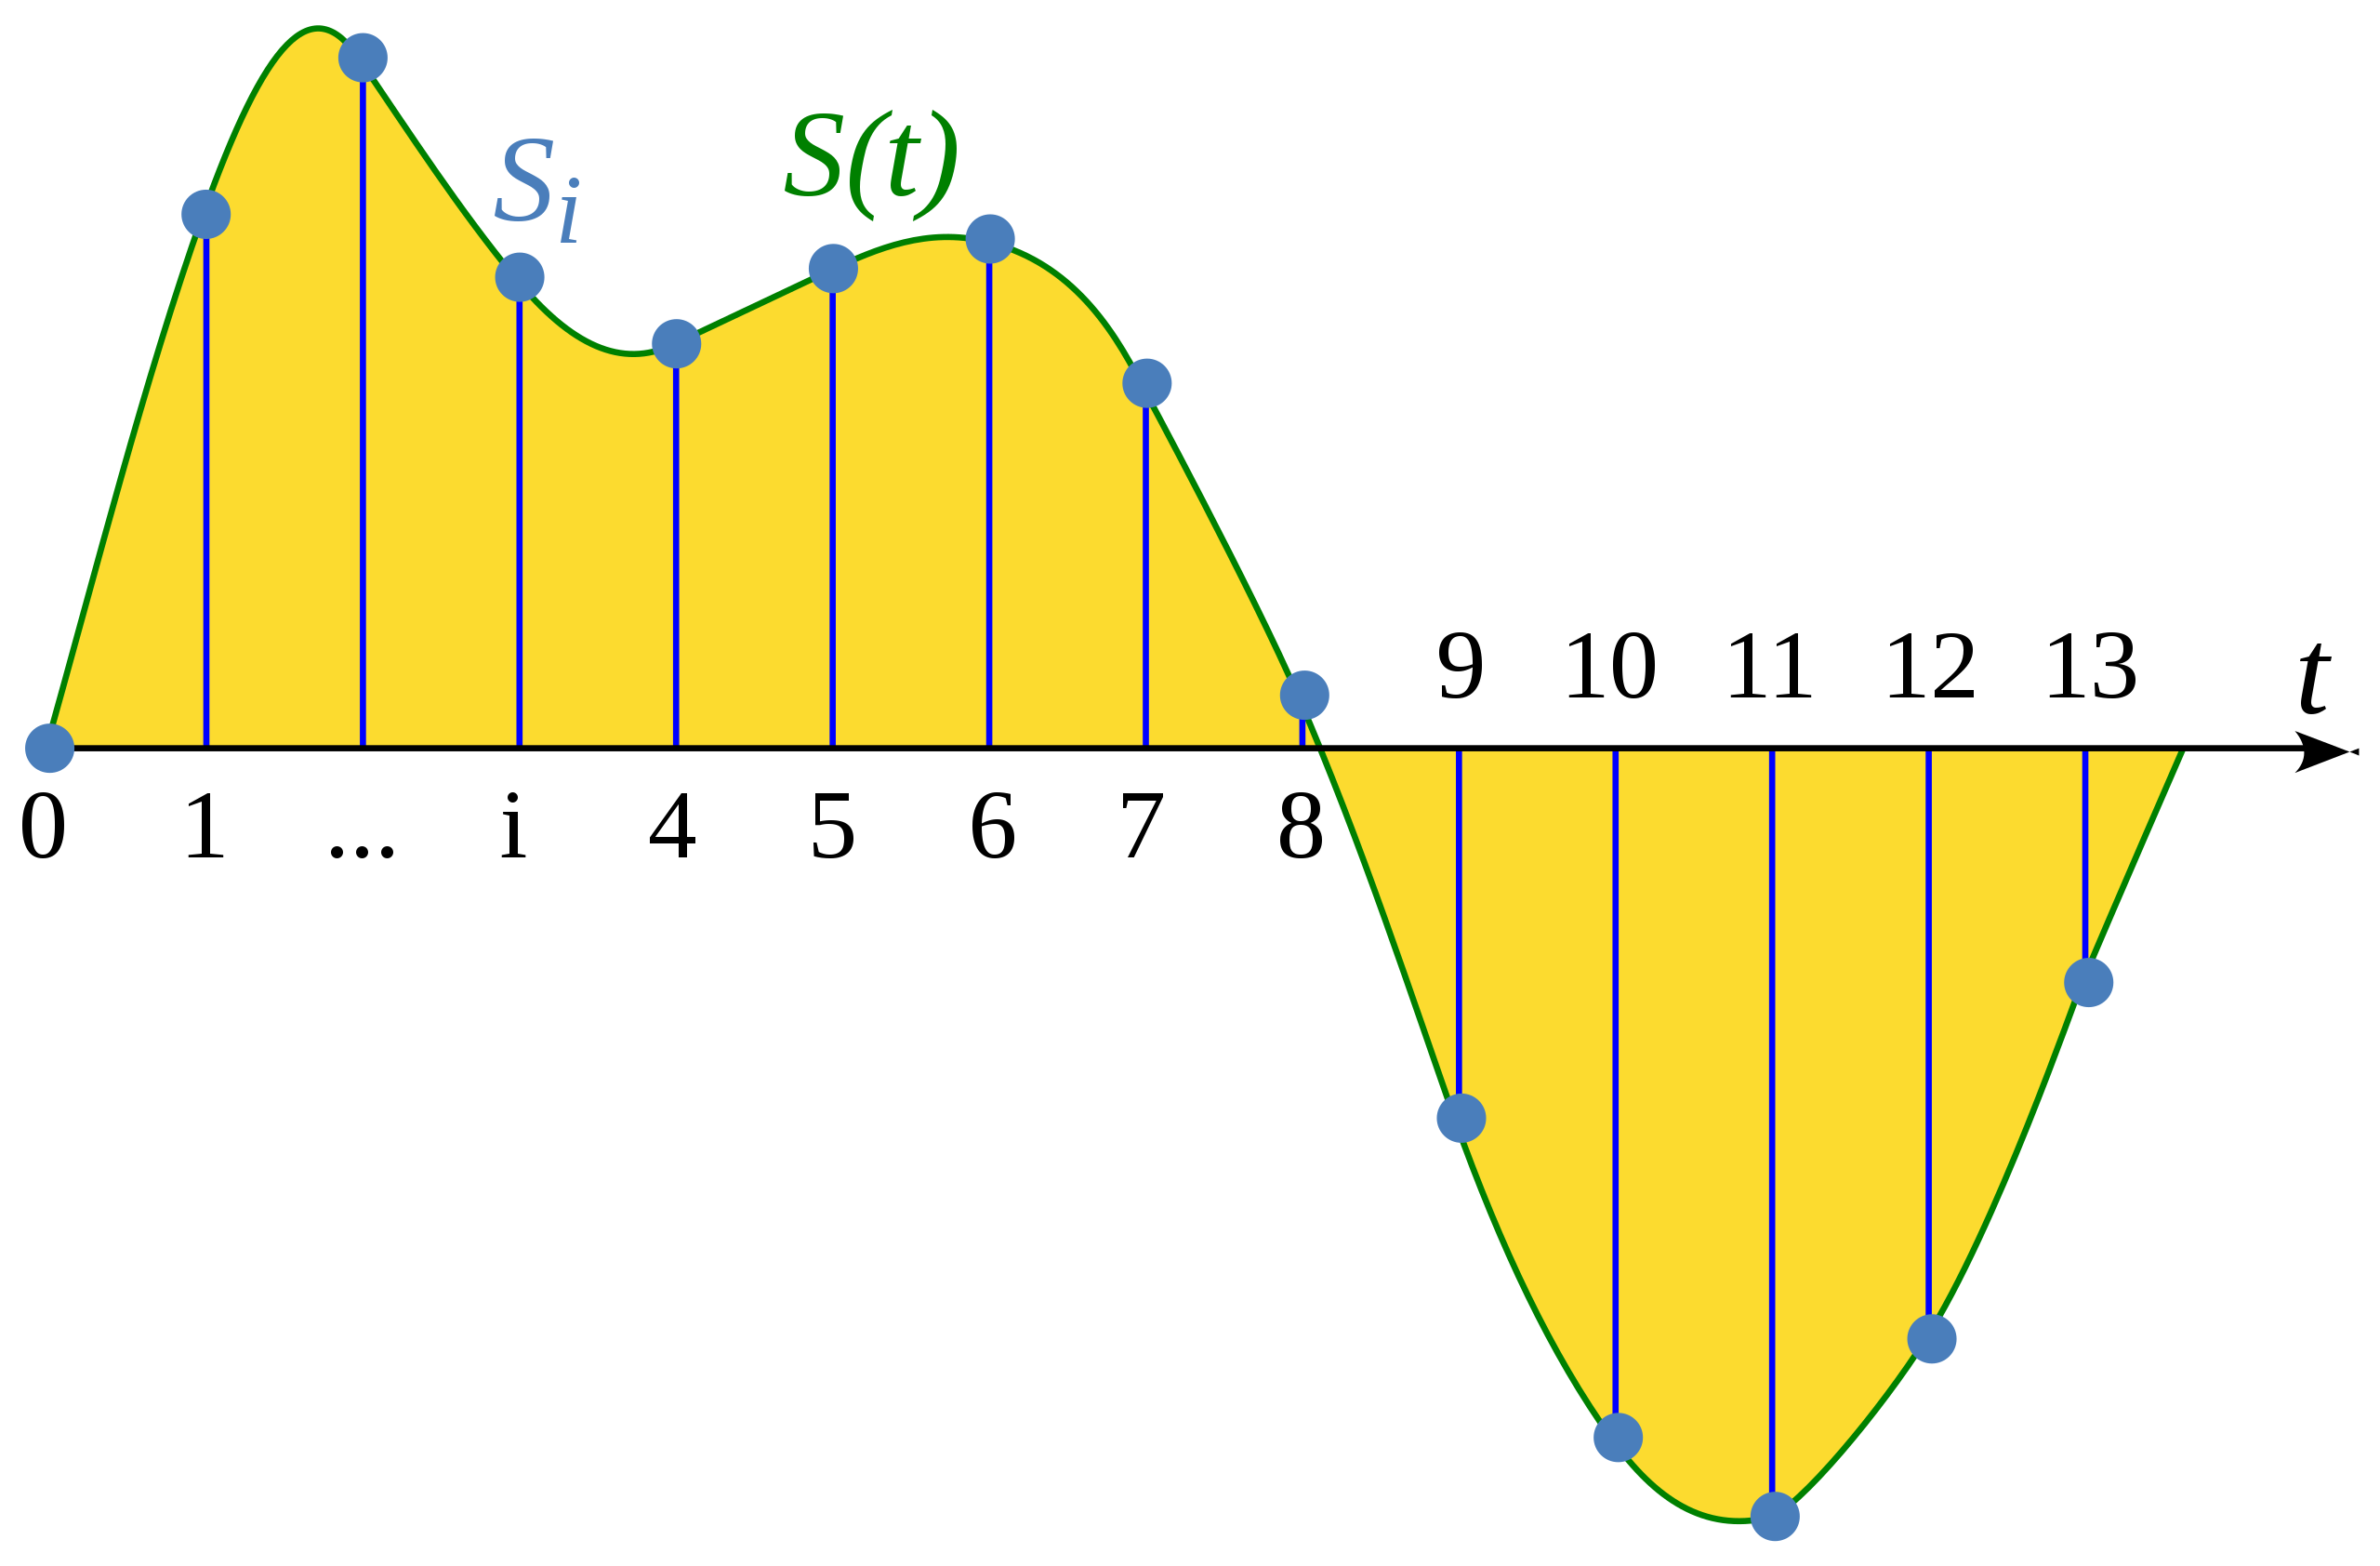
\includegraphics[scale=0.15]{discreth.png}
	\caption{Пример дискретизация непрерывного аналогового сигнала}
	\label{ris:discreth}
\end{figure}

Пример дискретизации показан на Рисунке 1.1.
\section{Квантование}
\quad
Квантование – это преобразование аналогового сигнала в ступенчатый сигнал с двоичным отсчетом уровней в квантах\cite{four}. При этой операции производится округление входного сигнала к принятой двоичной шкале квантователя. Процедуру квантования можно рассматривать как прохождение входного сигнала через устройство с амплитудной характеристикой ступенчатой формы (Рисунок \ref{ris:quant}), которая называется характеристикой (или шкалой) квантования. Если в пределах всей шкалы шаг квантования постоянен, то квантование называют равномерным. Такой вид квантования удобен для начального представления звукового сигнала с целью последующей обработки.
Пример квантования изображен на рисунке 1.3.
\clearpage
\begin{figure}[!htbp]
	\centering
	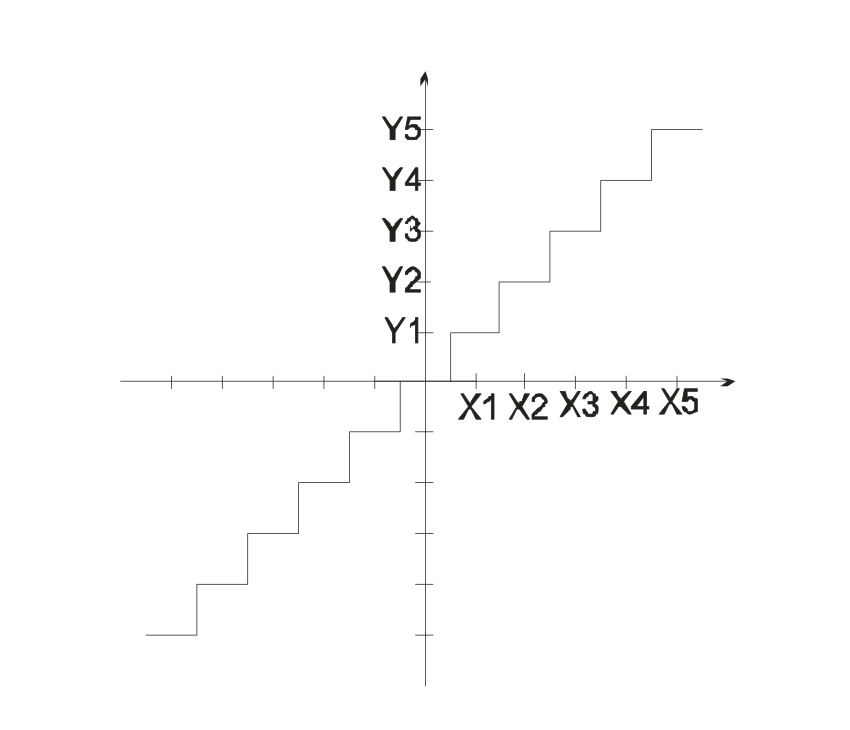
\includegraphics[scale=0.7]{quant.png}
	\caption{Характеристика квантования}
	\label{ris:quant}
\end{figure}

Максимальное число уровней для каждой полярности звукового сигнала определяется числом разрядов m :

\begin{equation}
	N_{KB} = 2^{(m-1)} - 1
	\label{eq:ref}
\end{equation}


При оцифровке сигнала количество битов, кодирующих один уровень квантования, называют глубиной квантования или разрядностью. Чем больше уровней квантования, тем на большее число ступеней разбивается шкала квантования и тем с большей точностью производится аналого-цифровое преобразование\cite{eight}. Но квантование сигналов неизбежно сопровождается погрешностью (или шумом квантования).

В звукотехнике в настоящее время наиболее распространены два вида квантования: импульсно-кодовая модуляция и сигма-дельта-модуляция.
\subsection{Импульсно-кодовая модуляция}
\quad

Импульсно-кодовая модуляция или PCM это особый тип метода аналого-цифрового преобразования, в котором данные или информация, содержащиеся в выборках аналогового сигнала, могут быть получены с помощью цифровых процедур. В этом методе каждый из цифровых сигналов имеет n двоичных цифр, есть M = $2^n$\cite{ten}.

Возможен уникальный номер кода, и все эти коды имеют определенный уровень амплитуды. Однако для каждой выборки значимость аналогового сигнала может быть люблй из неограниченных уровней.

Используется зашифрованное цифровым способом слово, амплитуда которого наиболее близка к фактическому значению выборки. Это называется квантованием, а процесс - квантованием. В качестве альтернативы использования аналогичного выборочного значения аналоговой формы w (кТс), ближайшее допустимое значение заменяет выборку, в которой имеется M разрешенных значений, каждое из которых соответствует одному из кодовых слов.

\begin{figure}[!htbp]
	\centering
	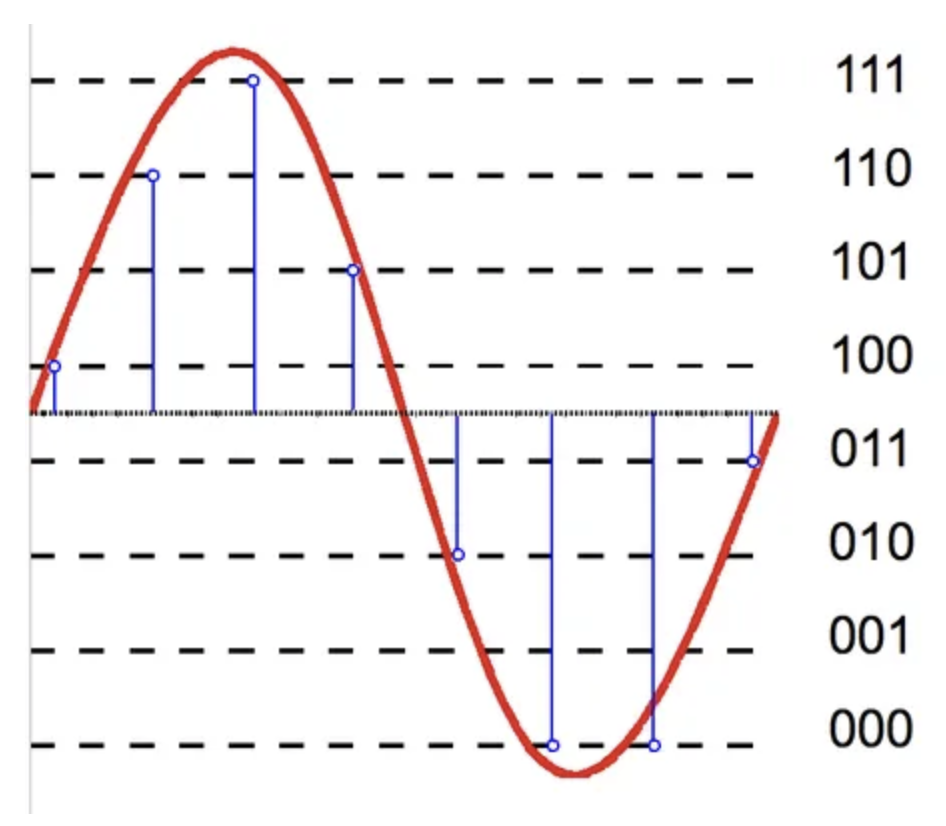
\includegraphics[scale=0.7]{impcodemod.png}
	\caption{Аналоговое сравнение с 3-битным разрешением}
	\label{ris:impcodemod}
\end{figure}

Модуляция с импульсным кодированием имеет различные особенности. Некоторые из важных особенностей импульсно-кодовой модуляции:
\begin{enumerate}
	\item техника ИКМ представляет собой сравнительно дешевую цифровую схему и может широко использоваться в различных приложениях;
	\item сигнал с импульсной кодовой модуляцией является результатом комбинации всех категорий аналоговых сигналов (видео, аудиовизуальные и т. Д.) С сигналом данных (т. Е. Доступным с цифровых компьютеров или портативных компьютеров) и передается по стандартной высокоскоростной цифровой схеме связи. Этот метод мультиплексирования называется TDM;
	\item в схемах удаленной цифровой связи, требующих ретрансляторов, чистый сигнал ИКМ восстанавливается на выходе каждого ретранслятора, где i / p состоит из импульса ИКМ, смешанного с шумом. Тем не менее, шум в i / p-сигнале может создавать битовые ошибки o / p в методе PCM;
	\item отношение сигнал / шум цифровой системы могло бы быть улучшено по сравнению с аналоговой системой. Вероятность ошибки в выводе системы можно было бы еще больше минимизировать, используя надлежащую методику шифрования на основе кодирования. Этим компенсируется главный недостаток ПКМ; требуется гораздо более широкий диапазон полосы пропускания, чем при использовании аналогичных аналоговых технологий.
\end{enumerate}

Сигнал импульсной кодовой модуляции генерируется из квантованного сигнала с амплитудно-импульсной модуляцией. Здесь кодируются квантованные значения. Как правило, разработчик системы назначается для того, чтобы указать одно и то же кодовое слово или шифрование, представленное конкретным квантованным уровнем для кода Грея. В этом результирующем сигнале импульсной кодовой модуляции это слово или байт для каждой квантованной выборки выводится из кодировщика следующим непосредственным импульсом. Код Грея используется, потому что в нем будет изменяться только один бит для каждого шага квантования. Как правило, «ошибки» в полученном сигнале ИКМ вызывают минимальные ошибки в полученном аналоговом сигнале при условии, что бит знака не является ошибочным.

Способы PCM иллюстрируют квантованное значение аналоговой выборки двоичными кодами. Как правило, существует вероятность определения квантованных аналоговых отсчетов с помощью цифровых слов с использованием базы, отличной от «2», или равномерно преобразовывать двоичный сигнал в другой многоуровневый сигнал.

В итоге Импульсно-кодовая модуляция имеет нижеперечисленные преимущества и недостатки.

Преимущества:
\begin{enumerate}
	\item PCM передает сигналы равномерно;
	\item PCM имеет эффективное оотнешение сигнал/шум;
	\item PCM всегда предлагает эффективную регенерацию.
\end{enumerate}

Недостатки:
\begin{enumerate}
	\item затухание происходит из-за шума и перекрестных помех;
	\item для передачи PCM требуется широкая пропускная полоса;
	\item при передаче наблюдаются ошибки.
\end{enumerate}

\subsection{Сигма-дельта модуляция}
\quad
Сигма-дельта модуляция предназначена для аналого-цифрового и цифро-аналогового преобразований звуковых сигналов. В отличие от импульсно-кодовой модуляции она позволяет использовать при этих операциях достаточно грубые преобразователи с числом разрядов вплоть до одного, обеспечивая при этом отношение сигнал шум (SNR) до 120...140 дБ, что необходимо для профессиональной записи звука\cite{eleven}.

Технология производства АЦП и ЦАП на основе сигма-дельта модуляции значительно проще и дешевле, поэтому такие преобразователи широко используются в современных звуковых картах, оптической звукозаписи, цифровых магнитофонах, в измерительной и другой технике. В отличие от ИКМ АЦП и ЦАП на основе сигма-дельта модуляции работают на частоте дискретизации в четыре и более раз выше стандартного значения, соответствующего требованиям теоремы В.П. Котельникова. В них используются грубые квантователи с числом разрядов q от 1 до 6 с частотно-зависимой отрицательной обратной связью\cite{twelve}.

В последние годы эта модуляция практически полностью «вытеснила» из бытовой и даже профессиональной аудиотехники импульсно-кодовую модуляция, поэтому ее изучение по дисциплине «Аудиовизульная техника» стало настоятельной необходимостью.

Модуляция сложная для понимания, даже автор этого изобретения не смог в своем патенте достаточно точно объяснить, как она работает. К сожалению, в технической литературе сигма дельта модуляция описывается либо очень примитивно на популярном уровне, либо слишком сложно с громоздкими математическими преобразованиями, недоступными большинству людей.

В сигма-дельта модуляторе используется двухуровневый квантователь типа midriser , на выходе которого логическая «1» если сигнал на его входе больше 0, и логический «0», если равно или меньше 0. D - триггер повторяет эти состояния с задержкой на один такт, и формирует двухуровневый, но однополярный цифровой поток. На выходе ЦАП логической «1» соответствует положительное опорное напряжение, а логическому «0»- отрицательное. Для декорреляции ошибок квантования с выходным ЗС может использоваться технология Dithering.

На счетный вход триггера подается частота fsk , с которой осуществляется дискретизация аналогового сигнала. Она обязательно выше частоты Найквиста. Интегратор создает частотную зависимость выходного звукого сигнала и ошибок квантования. Отрицательная обратная связь стремится уравнять выходной сигнал модулятора с входным.

В таком модуляторе выходной сигнал представляет собой непрерывную последовательность логических «1» и «0» одной полярности, в которой звуковой сигнал передается в виде модуляции плотности логических единиц, как среднее значение цифрового потока П-импульсов различной частоты и длительности. Этот цифровой поток называется DSD (Direct Stream Digital).

В таком потоке плотность логических «1» максимальна при амплитудах ЗС положительной полярности, а плотность логических «0» максимальная при амплитудах звукового сигнала отрицательной полярности. При значениях звукового сигнала близких к нулю, плотности логических «1» и «0» одинаковые и минимальны.
Рассмотренный модулятор называется аналоговым и он используется в АЦП (Рисунок \ref{ris:anmod}). В ЦАП применяется цифровой модулятор. От аналогового модулятора он отличается тем, что преобразует в цифровой поток DSD, подаваемый на его вход, много разрядный цифровой сигнал с высокой частотой дискретизации fsk.

\begin{figure}[!htbp]
	\centering
	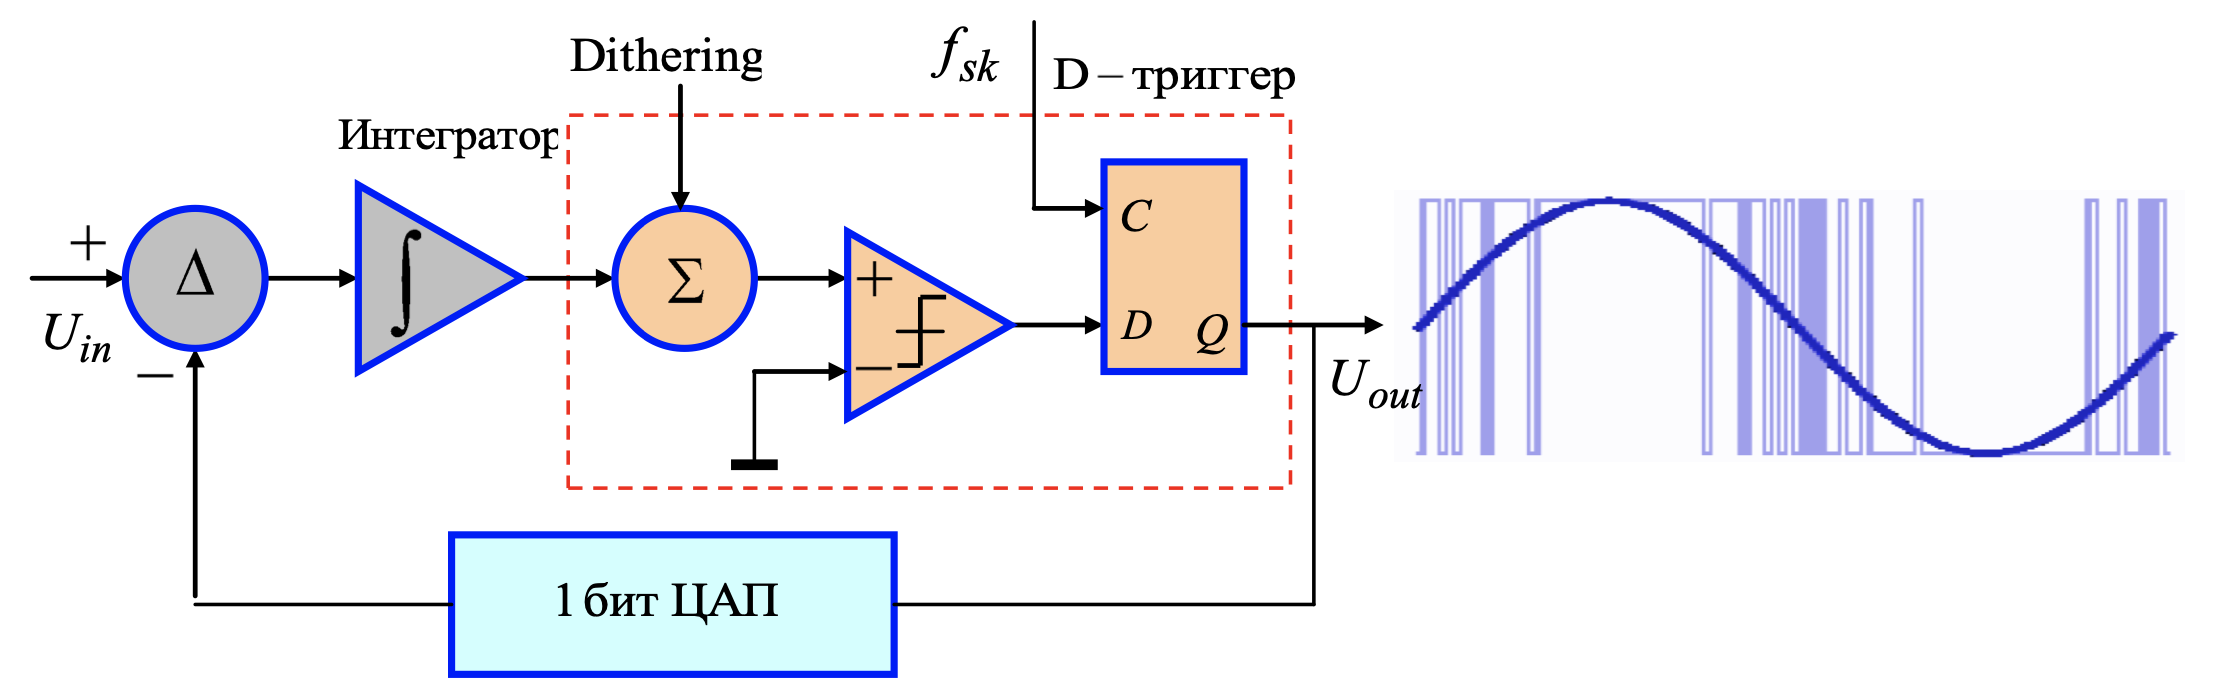
\includegraphics[scale=0.4]{anmod.png}
	\caption{Функциональная схема 1-бит аналогового сигма-дельта модулятора}
	\label{ris:anmod}
\end{figure}


В соответствии с теоремой Найквиста (В.П.Котельникова) частота дискретизации должна быть, по крайней мере, вдвое выше максимальной частоты спектра звукового сигнала. Эта частота называется частотой Найквиста. Преобразование аналоговых сигналов в цифровые осуществляется с помощью двух типов квантователей: Mid-Tread и Mid-Riser.

Квантователь Mid-Tread используется при импульсно-кодовой модуляции и многоразрядной сигма-дельта модуляции. У него всегда нечетное число уровней квантования, определяемое равенством (1.4).

\begin{equation}
	N_{KB} = 2^{(q)} + 1
	\label{eq:ref}
\end{equation}

Минимально может быть только 3 уровня:0, $\Delta$, -$\Delta$.

Квантователь имеет отсечку, равную половине шага квантования. Пока пиковое значение входного сигнала не превысит этого значения, на выходе квантователя сигнал отсутствует. Поэтому он не может использоваться как одноразрядный. Для линеаризации передаточной характеристики многоразрядного квантователя Mid-Tread необходимо использовать технологию Dithering.

Квантователь типа Mid-Riser используется только при одноразрядной сигма дельта модуляции. У него число уровней квантования определяется равенством (1.5).
\begin{equation}
	N = 2^q
	\label{eq:ref}
\end{equation}

Оно всегда четное число и минимально может быть два уровня: +$\Delta$/2, -$\Delta$/2.

Следует различать и не путать ошибки округления и ошибки квантования. Разность между аналоговым $U(t)$ и квантованным $U(t)_q$ сигналами называется ошибкой округления (равенство 1.6).

\begin{equation}
	e(j)_r = U(t) - U(t)_q
	\label{eq:ref}
\end{equation}

Ошибка квантования - разность мгновенных значений дескритизированного $U(j)_d $ и квантованного сигналов $U(j)_q$ в моменты выборки $e(j)$, нет операции дискретизации - нет ошибок квантования.

\begin{equation}
	e(j)_q = U(t)_d - U(t)_q
	\label{eq:ref}
\end{equation}

Ошибки квантования возникают при аналого-цифровом преобразовании, но проявляются при цифро-аналоговом преобразовании в ЦАП, где с помощью УВХ (устройство выборки и хранения) они сохраняются от одной выборки до другой\cite{thirty}. Ошибки округления это ошибки квантования при очень высокой частоте дискретизации (Рисунок \ref{ris:mistakes}).

\begin{figure}[!htbp]
	\centering
	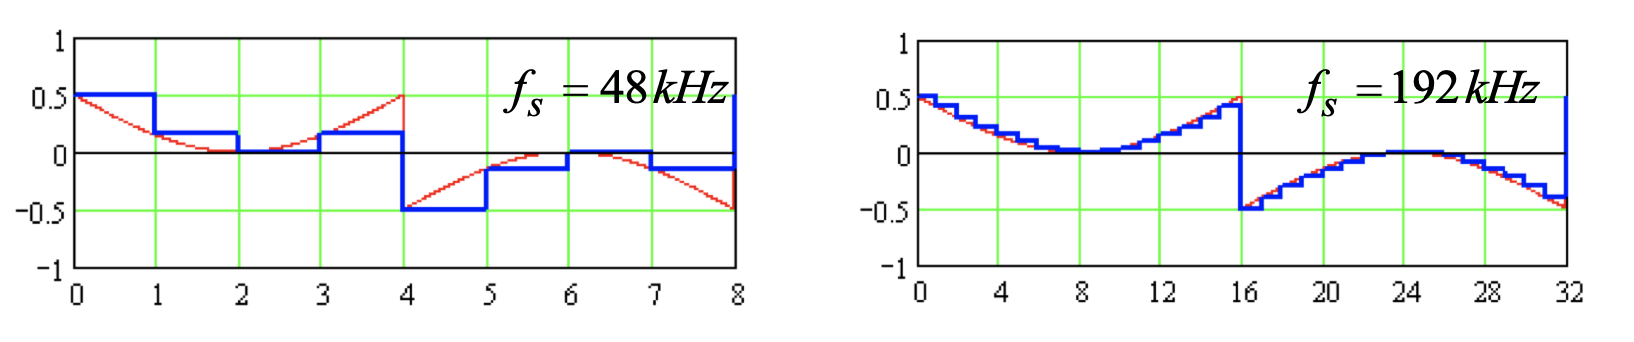
\includegraphics[scale=0.6]{mistakes.png}
	\caption{Ошибки округления (красный) и квантования (синий) при разных частотах дискретизации}
	\label{ris:mistakes}
\end{figure}

Таким образом, ошибки квантования это дискретизированные ошибки округления. С повышением частоты дискретизации разница между этими ошибками стремится к нулю. Ошибки округления достаточно просто рассчитываются, а ошибки квантования не поддаются математическому описанию, так как они очень сложным образом зависят от уровня, частоты и формы звукового сигнала. Поэтому часто, неправильно, ошибки округления называют ошибками квантования.

Спектр ошибок округления и квантования дискретный, в частности, при частоте дискретизации кратной частоте звукового сигнала он представляет собой медленно затухающие гармоники звукового сигнала(Рисунок \ref{ris:mistakes2}). Отличие этих двух ошибок в том, спектр ошибок квантования не превышает частоты Найквиста, и при стандартных частотах дискретизации он полностью попадает в звуковой диапазон и слышен в виде призвуков или шума. Спектр ошибок округления не ограничен по частоте. Он всегда состоит из бесконечного числа очень медленно затухающих гармоник звукового сигнала.

В зависимости от характера звукового сигнала ошибки квантования могут быть детерминированными, то есть сильно коррелированными со звуковым сигналом, или случайными, не связанными со звуковым сигналом. Это может быть, когда звуковой сигнал является музыкальным. С помощью специальных аудио технологий детерминированные ошибки квантования могут быть преобразованы в случайные. У случайных ошибок спектр сплошной и он простирается также до частоты Найквиста.
Вся теория квантования хорошо разработана применительно к квантователю Mid-Tread в предположении, что входной сигнал по уровню много больше шага квантования и является стационарным случайным процессом с равномерной плотностью вероятности ошибокквантования в диапозоне $\pm\Delta/2$.

При таких условиях ошибки квантования имеют характер белого шума, пиковые значения которого не превышают половины шага квантования. Основными характеристиками такого шума является мощность шума квантования $P_q$ и спектральная плотность мощности $S_d$ . Она определяется как отношение мощности $P_q$ к ширине спектра шума квантования от 0 до частоты Найквиста (равенство 1.8).

\begin{equation}
	S_d = \frac{P_q}{f_n}
\end{equation}

Для  звуковых сигналов, которые по уровню значительно выше шага квантования, мощность шума квантования равна $\Delta^2/12$. Она не звасисит от уровня звукового сигнала, его частоты и частоты дискретизации. Отношение сигнала шум квантователя этого типа определяется равенством 1.9.

\begin{equation}
	SNR_q = 6,02q + 1,76dB
\end{equation}

Одноразядный квантователь Mid-Riser не имеет отсечки и поэтому принципиально линеен. Однако, отсутствие отсечки приводит к тому, что при любом минимальном уровне шума на входе квантователя на его выходе создается квантованный шум с пиковыми значениями $\Delta/2$. Тем не менее, во всех публикациях по расчету отношения сигнал/шум такого квантователя принимается, что мощность его шума также равна $\Delta^2 /12$.

\begin{figure}[!htbp]
	\centering
	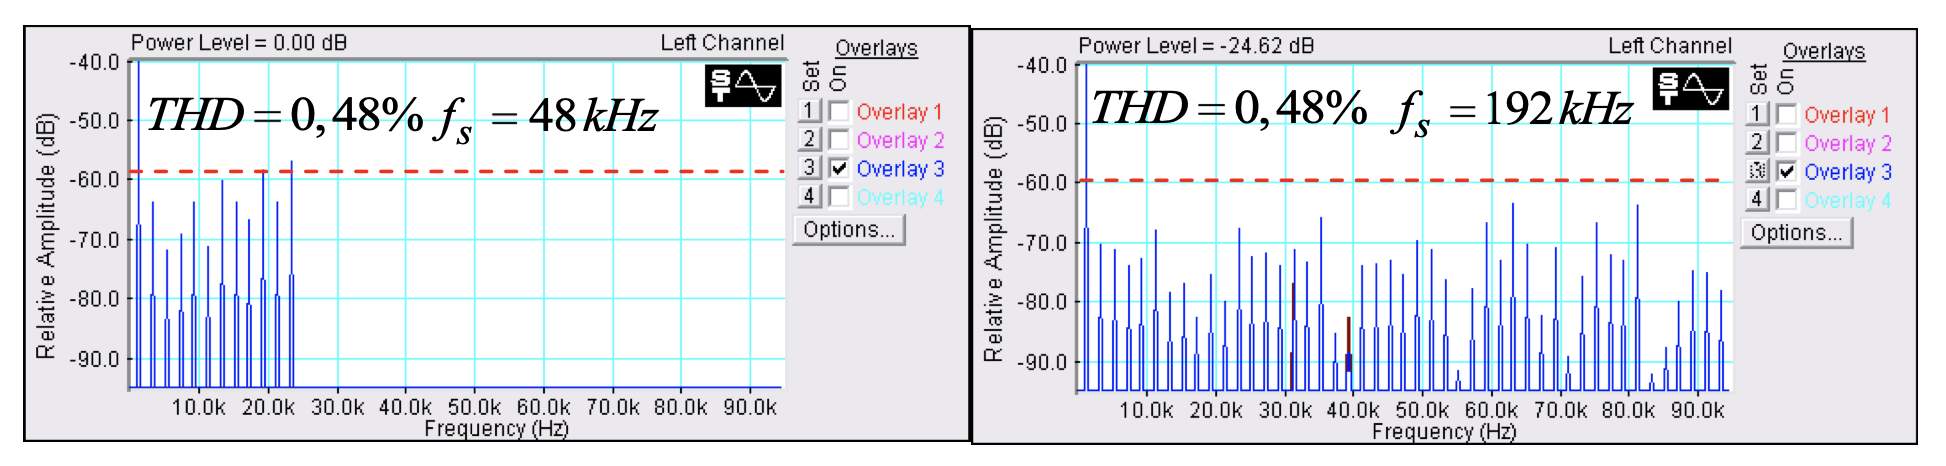
\includegraphics[scale=0.5]{mistakes2.png}
	\caption{Спектры ошибок квантования при двух частотах дискретизации}
	\label{ris:mistakes2}
\end{figure}

Важной отличительной особенностью сигма дельта-модуляции является одновременное использование трех аудио технологий: Dithering, Oversampling и Noise Shaping\cite{fifty}. С помощью этих технологий ошибки квантования преобразуются в шум, спектр шума расширяется в область ультразвуковых частот и преобразуется так, что его спектральная плотность мощности в звуковом диапазоне сильно уменьшается, а в области высоких частот далеко за пределами частоты Найквиста увеличивается.

\chapter{Классификация существующих форматов сжатия аудиофайлов}
\quad
Из-за большой разновидности применения и требования к аудиофайлам, существует множество форматов сжатия, однако их можно поделить на три основные группы:
\begin{enumerate}
	\item аудиоформаты без сжатия;
	\item аудиоформаты со сжатием без потерь;
	\item аудиоформаты со cжатием с потерями;
\end{enumerate} 

Так же в отдельную группу можно выделить модульные музыкальные форматы файлов, так как в них аудио создается синтетически или из семплов заранее записанных живых инструментов. Они в основном служат для создания современной электронной музыки.

В данной нучно-исследовательской работе будут рассмотрены аудио форматы с сжатием с и без потерь, а также один аудиоформат без сжатия, а именно WAV.

\section{Аудиоформат без сжатия}
\quad 
Самым известным и широко поддерживаемым аудиоформатом без сжатия является WAV, так как он изначально использовался в операционной системе Windows для сохранения цифровых аудиоданных и для WAV было написано большое количество программ. Так же практически любая современная программа для работы с цифровым звуком поддернживает работу с WAV. 

В случае с форматом WAV звук записывается довольно простым способом: входящий звуковой поток разбивается на малейшие отрезки (кванты, отсюда термины «частота квантования», «частота выборки» или "частота дискретизации") и в каждый такой отрезок времени пишется текущее значение аналогового сигнала в двоичной форме\cite{six}. Так же из-за этого очень легко работать с WAV файлами не только в программах для создания или обработки музыки, но и на совершенно не отнасящихся к музыке программах, таких как matlab (Рисунок 2.1). Файлы формата WAV могут быть записаны с частотой дискретизации, к примеру, от 8 кГц до 192 кГц, но стандартом считается частота выборки в 44.1 кГц. 

\begin{figure}[!htbp]
	\centering
	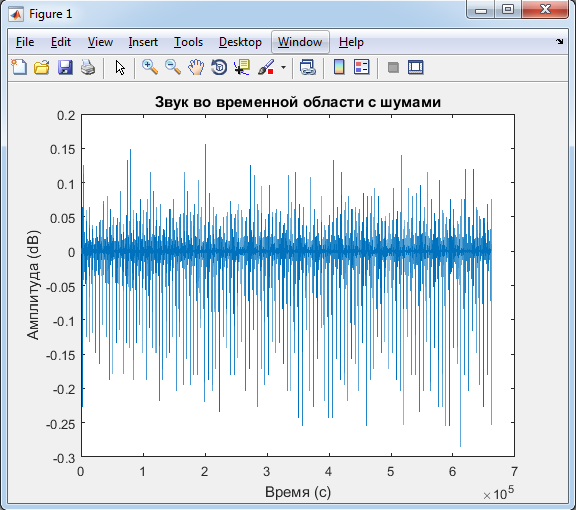
\includegraphics[scale=0.7]{wavgraph.png}
	\caption{Визуализация wav-файла в виде волны во временной области в matlab}
	\label{ris:wavgraph}
\end{figure}

Частота 44.1 кГц произошла не случайно. Если допустить неточности в описании, то данная цифра произошла как утверждение теоремы Котельникова: для сохранения максимально правильной формы волны при частотах до 20 кГц (теоретический предел слышимости человеческого уха) необходима частота дискретизации вдвое выше — 40 кГц. Собственно, частота именно в 44.1 кГц обусловлена техническими аспектами. Следует отметить, что WAV, как контейнер, поддерживает и другие способы хранения аудио-информации: к примеру, ADPCM, который способен, в зависимости от полосы пропускания, кодировать аудио-данные с переменной частотой дискретизации.

Как отмечалось выше, самыми распространенными методами квантования являются импульсно-кодовая модуляция и сигма-дельта модуляция, ADPCM, она же адаптивная дифференциальная импульсно-кодовая модуляция является разновидность импульсно-кодовой модуляции, алгоритм которой подразумевает изменение шага квантования, что позволяет снизить требуемую полосу пропускания для заданного отношения сигнал/шум. Обычно адаптация основывается на адаптивном коэффициенте масштабирования.Алгоритм ADPCM был разработан в начале 1970-х годов П. Каммиски, Н. С. Джаянт и Джеймсом Л. Фланаганом в Bell Labs для кодирования голоса.

Возвращаясь к "классическому" WAV, в каждом отрезке в двоичной форме кодируется фактическое напряжение аналогового сигнала: высший уровень можно представить в виде «1111», низший — в виде «0000». И вот здесь имеет важность второй параметр — глубина звучания, определяющая, насколько точно будет оцифровано значение волны в отрезок времени. Зачастую файлы формата WAV пишутся с разрядностью в 16 бит или 32 бит. Выше разрядность — точнее запись.

Из всего вышеперечисленного можно сделать следующие выводы о формате аудиофайлов WAV:
\begin{enumerate}
	\item самое высокое качество звука, так как отсутсвует сжатие и в файл записывается максимально полная информация о звуке;
	\item из-за отсутствия сжатия и того, что в файл записывается все, файл занимает много памяти;
	\item WAV широко поддерживается и из-за этого с ним относительно легко работать, в сравнении с другими форматами;
	\item музыка в формате WAV подходит для тех, кто хочет слушать действительно качественную музыку со всеми деталями.
\end{enumerate}

\section{Аудиоформаты со сжатием без потерь} 
\quad
Так как аудиофайлы занимают много памяти, а хранение большого количества музыки это дорого, а также из-за скорости передачи этих файлов в сети, аудиофайлы научились сжимать, обрезая ненужную информацию и ту информацию, котороя может некретично изменить звучание. Однако это используют не все, потому что мало кому хотелось бы послушать классическую композицию Бетховена, где все инструменты в самый напряженный момент просто превращаются в кашу, именно поэтому было изобретено сжатие без потерь, которое уменьшает размер файла и практически не изменяет его звучание.
Двое из самых популярных таких форматов это FLAC и OptimFROG.
\subsection{FLAC}
FLAC является кодеком для сжатия аудио данных, изначально написанный Джошем Колсоном. Как следует из названия, Free Lossless Audio Codec, FLAC осуществляет сжатие данных, оставляя при этом их идентичными оригиналу, таким образом, ни одна часть данных не теряется — это и является основной задачей алгоритмов сжатия без потерь. Цифровая аудио запись (такая как CD-Audio трэк), сжатая в формат FLAC может быть распакована в абсолютно идентичную копию аудио данных. Степень сжатия формата FLAC, как правило, варьируется от 50 до 60 процентов от оригинального размера\cite{two}. На рисунке 2.2 изображена запущенная программа (кодек) FLAC.

\begin{figure}[!htbp]
	\centering
	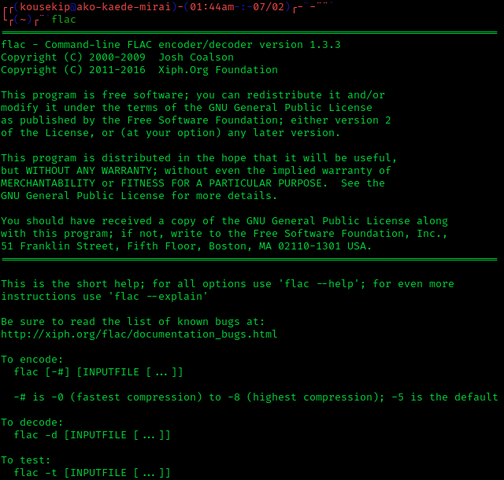
\includegraphics[scale=0.6]{flaccodec.png}
	\caption{Запущенный кодек FLAC}
	\label{ris:flaccodec}
\end{figure}

FLAC подходит как для ежедневного прослушивания записей, так и для архивирования. Бесплатность и открытость формата делают его хорошо поддерживаемым различным программным обеспечением. Поддержка воспроизведения на различных устройствах достаточно ограничена на данный момент, но, тем не менее, формат поддерживается большим количеством аппаратных устройств по сравнению с конкурирующим форматом WavPack.

Разработка была начата в 2000-м году Джошем Колсоном. Формат битового потока был зафиксирован, когда FLAC вошел в бета стадию с версией 0.5, выпущенной 15 января 2001 года. Версия 1.0 была выпущена 20 июля 2001 года.

29 января 2003 года организация Xiph.Org и проект FLAC объявили о включении проекта FLAC под символ Xiph.Org.

17 сентября 2007 года была выпущена версия 1.2.1, в которой была добавлена возможность сохранять AIFF и RIFF цепочки метаданных при помощи ключа --keep-foreign-metadata.

Спустя 6 лет 26 мая 2013 года вышел следующий релиз 1.3.0 от новой команды Xiph.Org. В этот релиз вошли небольшие изменения и общие улучшения. В частности, проект переехал в git-репозиторий организации Xiph.Org и была добавлена поддержка форматов RF64 и Wave64.

После прошествия ещё полутора лет 25 ноября 2014 года вышел в свет релиз 1.3.1 с более серьезными изменениями. В этот раз была улучшена производительность кодирования при использовании SSE и AVX расширений. Также была улучшена производительность декодирования для всех разрядностей, но особенно для 24 бит в связке с архитектурой IA32.
FLAC использует линейное прогнозирование для конвертации сэмплов в небольшие последовательности некоррелирующих чисел (известных как остаточные), которые хранятся используя эффективное кодирование Голомба-Райса. Также в формате FLAC используется кодирование блоков с идентичными сэмплами, таких, как тихие пассажи. Технической силой формата FLAC, по сравнению с другими кодеками без потерь, является его возможность быть потоковым и декодироваться за короткое время, которое не зависит от степени сжатия.

Будучи схемой сжатия без потерь, FLAC также является популярным форматом для хранения архивов у владельцев аудио дисков или других медиа-данных, стремящихся сохранить свою аудио коллекцию. Если оригинальная запись потеряется, повредится или износится, копия в формате FLAC дает гарантию того, что точный дубликат оригинальной записи может быть восстановлен в любое время. Точное восстановление из архива с потерями невозможно. Являясь форматом без потерь, FLAC вполне может подвергаться транскодингу без потерь качества, как правило, свойственным транскодингу. Во время извлечения данных с CD может быть также создан CUE файл. Если данные с компакт диска были извлечены в формат FLAC успешно, то файл CUE позволяет восстановить копию диска, идентичную оригинальному, включая порядок треков, начальный зазор (pregap) и CD-Text данные. Однако, дополнительная информация, которая может присутствовать на некоторых аудио дисках, такая как тексты песен, графика CD+G будут находиться за полем видимости CUE файла и большинства извлекающего программного обеспечения, и, таким образом, эта информация не будет извлечена.

Европейский вещательный союз (EBU) принял на вооружение формат FLAC для распространения высококачественного звука через сеть «Еврорадио».

Формат FLAC поддерживает только целочисленные сэмплы. Это позволяет избежать неточностей нецелочисленной арифметики, таким образом, это дает гарантию сжатия без потерь. На вход кодировщик может принимать от 4 до 32 бит на сэмпл, любую частоту дискретизации от 1 Гц до 655 350 Гц с шагом в 1 Гц, а также любое количество каналов в диапазоне от 1 до 8. Каналы могут быть сгруппированы в случае стерео или 5.1 звука для извлечения выгода от межканальных корреляций и, тем самым, увеличивая степень сжатия звука. FLAC проверяет контрольные суммы CRC для обнаружения испорченных фреймов в тех случаях, когда формат используется в потоковом протоколе. Помимо этого, в тэге с заголовком STREAMINFO хранится полный MD5 хэш необработанных PCM аудио данных. FLAC допускает диапазон Rice параметра от 0 до 16. FLAC поддерживает ReplayGain.

FLAC реализован как ядро кодека в библиотеке libFLAC, которая слинкована с основной поставляемой программой flac, являющейся эталонной программой, использующей API libFLAC. Также API кодека доступно для C++ в библиотеке libFLAC++.

Эталонная реализация FLAC компилируется на многих платформах, включая системы Unix (такие как Solaris и Mac OS X) и Unix-подобные (включая Linux и BSD), Windows BeOS и OS/2. Проект настроен для сборки следующими утилитами: autoconf / automake, MSVC, Watcom C и Xcode. В настоящий момент FLAC не поддерживает многопоточность.

Для тэгов FLAC использует ту же систему, что и Vorbis-комментарии.

Из всего вышеперечисленного можно сделать следующие выводы о формате аудиофайлов FLAC:
\begin{enumerate}
	\item высокое качество звука, но хуже чем у WAV;
	\item исходный код открыт и легко лицензирован;
	\item быстрое декодирование, высокая независимость от уровня сжатия;
	\item поддержка стримминга;
	\item испорченные файлы могут быть частично восстановлены;
	\item коэфициент производительность/сжатие немного хуже чем у других современных форматов сжатия;
	\item довольно широкая поддержка;
	\item средний коэффициент сжатия, из-за чего файлы занимают не так много памяти как WAV, но и не настолько мало как у форматов со сжатием с потерями.
\end{enumerate}
\subsection{OptimFROG}
OptimFROG — это алгоритм сжатия без потерь, главная цель которого — максимально уменьшить размер аудио файлов. Это чем-то напоминает ZIP сжатие, но этот алгоритм высоко специализирован для аудио данных.

OptimFROG имеет один из лучших показателей сжатия аудио. Реализован на платформах Windows, Linux, Mac, имеет полнофункциональные плагины для Windows Media Player, foobar2000, Winamp2/3/5, dBpowerAMP, XMPlay, QCD и XMMS (со стойкостью к ошибкам в потоке данных, поддержкой чтения тегов ID3v1.1 и APEv2, и совместимостью с ID3v2). Присутствует оптимальная поддержка для всех целочисленных PCM форматов вплоть до 32 бит. Он так же быстр: стандартный режим кодирует информацию со скоростью 12.4x относительно реального времени и декодирует со скоростью 17.4x на процессоре AMD Athlon XP 1800+ (самый быстрый режим кодирования достигает результатов 28.1x и 24.7x соответственно). Также можно создавать самораспаковываемые архивы, с небольшим довеском к файлу в 54 КБ.

Сжатый по размеру получается от 25 процентов (тихая классическая музыка) до 70 процентов (шумная рок музыка) относительно оригинала. Это не идет в сравнение с MP3 (13 процентов), зато вы получаете идентичную копию оригинальных файлов.

OptimFROG использует новую технологию аудио сжатия: концепцию декорелляции стерео (совместно с оптимальным предсказателем), которая была введена в OptimFROG начиная с версии 4.0b (декабрь 2001). Благодаря этому нововведению, новая технология позволила достичь значительного улучшения (~1.5 процента) сжатия по сравнению с существующими показателями аудио кодеков без потерь. Сравнение скорости приведено на рисунке 2.3.

\begin{figure}[!htbp]
	\centering
	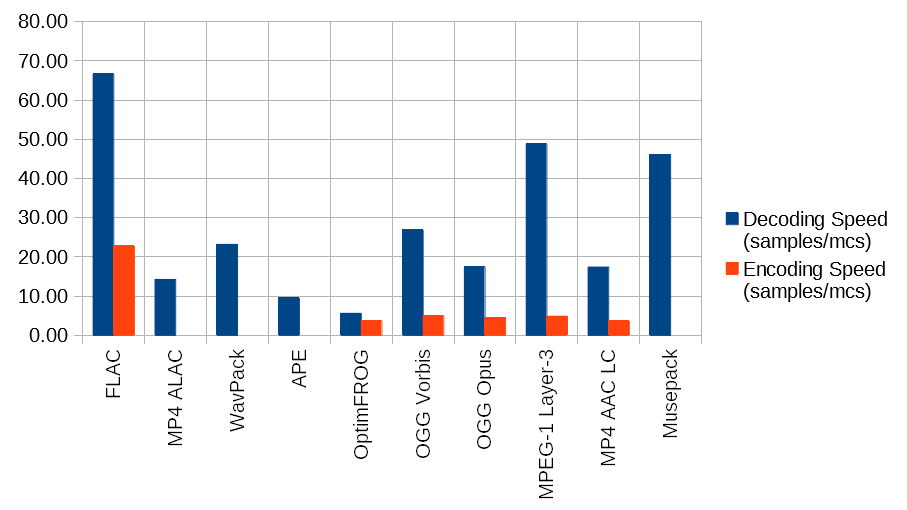
\includegraphics[scale=0.5]{optifrogbest.png}
	\caption{Сравнение скоростей кодирования/декодирования различных кодеков}
	\label{ris:optifrogbest}
\end{figure}

Автор Ghido активно развивал проект до 3 июля 2006 года, вплоть до версии 4.600ex. Затем последовал очень большой перерыв и, казалось, что на этом проект будет заброшен.

Версия 4.910b

Через почти 5 лет, 12 февраля 2011 года разработчик проекта решил выпустить очередную версию 4.910b. В ней была сохранена обратная совместимость, слегка улучшена степень сжатия, добавлен режим работы с некорректным заголовком WAV файлов.

Версия 5.000

Спустя ещё 4 года, 19 июня 2015 года вышел большой релиз 5.000. В нём лицензия проекта сменилась на менее строгую, разрешающую комменрческое использование и редистрибуцию. В дополнение к этому добавились официальные сборки Win/x64, OSX/x86+SSE2 и OSX/x64. Был значительно переработан платформозависимый код и внесено множество улучшений производительности. Размеры итоговых сжатых файлов остались идентичны версии 4.910b.

Из всего вышеперечисленного можно сделать следующие выводы о формате аудиофайлов OptimFROG:
\begin{enumerate}
	\item высокое качество звука, но хуже чем у WAV;
	\item самые высокие скорости кодирование/декодирования по сравнению с другими форматами сжатия без потерь;
	\item средний уровень поддержки;
	\item хороший коэффициент сжатия, из-за чего файлы занимают значительно меньше памяти чем у WAV, но не настолько мало как у форматов со сжатием с потерями.
\end{enumerate}

\section{Аудиоформат со сжатием с потерями}
\quad
Аудио со сжатием с потерями решает одну из главных проблем цифровых аудиофайлов, а именно размер файлов. Но с этим появляется другая проблема, качество звука, так как при большом сжатии невозможно сохранить исходное качество звука.

Однако данные форматы ранее пользовались огромной популярностью из-за размера, скорости передачи и того, что качественных средств для прослушивания музыки было не так много и далеко не у всех.

Самый популярный и известный из таких форматов это MP3.
\subsection{MP3}
\quad
MP3 разработан рабочей группой Института Фраунгофера под руководством Карлхайнца Бранденбурга и университета Эрланген-Нюрнберг в сотрудничестве с Bell Labs и Thomson.

Основой разработки MP3 послужил экспериментальный кодек ASPEC (Adaptive Spectral Perceptual Entropy Coding). Первым кодировщиком в формат MP3 стала программа L3Enc, выпущенная летом 1994 года. Спустя один год появился первый программный MP3-плеер — Winplay3.

При разработке алгоритма тесты проводились на вполне конкретных популярных композициях. Основной стала песня Сюзанны Веги «Tom’s Diner». Отсюда возникла шутка, что «MP3 был создан исключительно ради комфортного прослушивания любимой песни Бранденбурга», а Вегу стали называть родителем MP3.

Почти полный стандарт появился в открытом доступе 6 декабря 1991 года.

23 апреля 2017 года истекли последние патенты на формат и были прекращены сборы лицензионных отчислений с производителей программного обеспечения и встраиваемых решений. О прекращении лицензирования формата сообщил Институт Фраунгофера на своём официальном сайте. И, хотя формат mp3 всё ещё весьма популярен среди пользователей, большинство радиостанций и телеканалов перешли на использование современных кодеков, обеспечивающих лучшее сжатие и меньшую потерю качества звука.

Как и формат JPEG, MP3 использует спектральные отсечения, согласно психоакустической модели. Звуковой сигнал разбивается на равные по продолжительности отрезки, каждый из которых после обработки упаковывается в свой фрейм (кадр)\cite{three}. Разложение в спектр требует непрерывности входного сигнала, в связи с этим для расчётов используется также предыдущий и следующий фрейм. В звуковом сигнале есть гармоники с меньшей амплитудой и гармоники, лежащие вблизи более интенсивных — такие гармоники отсекаются, так как среднестатистическое человеческое ухо не всегда сможет определить присутствие либо отсутствие таких гармоник. Такая особенность слуха называется эффектом маскировки. Также возможна замена двух и более близлежащих пиков одним усреднённым (что, как правило, и приводит к искажению звука). Критерий отсечения определяется требованием к выходному потоку. Поскольку весь спектр актуален, высокочастотные гармоники не отсекаются, как в JPEG, а только выборочно удаляются, чтобы уменьшить поток информации за счёт разрежения спектра. После спектральной «зачистки» применяются математические методы сжатия и упаковка во фреймы. Каждый фрейм может иметь несколько контейнеров, что позволяет хранить информацию о нескольких потоках (левый и правый канал либо центральный канал и разница каналов). Степень сжатия можно варьировать, в том числе в пределах одного фрейма\cite{five}. Это одна из причин почему MP3 занимает меньше памяти и имеет более плохое звучание. Другая причина столь малого размера файлов MP3 и его некачественного звука, это битрейт, его максимальное значение меньше в три раза. Интервал возможных значений битрейта составляет 8—320 кбит/c. Наглядная разница в  количестве и точности сигналов между MP3 и форматами сжатия без потерь и без сжатия показана на рисунке 2.4.

\begin{figure}[!htbp]
	\centering
	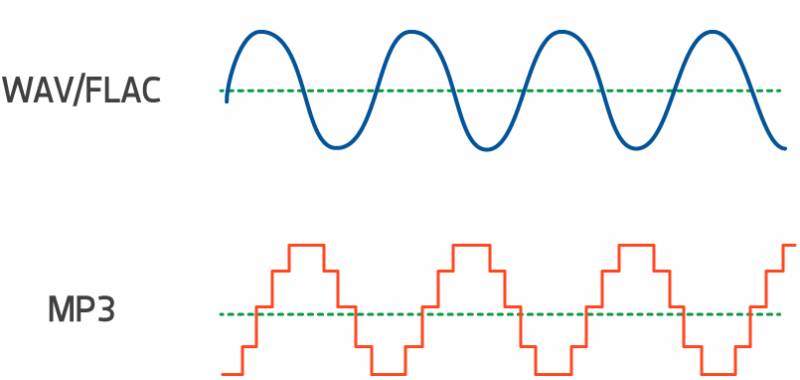
\includegraphics[scale=0.5]{mp3kek.png}
	\caption{Сравнение WAV/FLAC и MP3}
	\label{ris:mp3kek}
\end{figure}

Из всего вышеперечисленного можно сделать следующие выводы о формате аудиофайлов MP3:
\begin{enumerate}
	\item качество звука ниже среднего;
	\item низкая скорость декодирования и высокая скорость кодирования;
	\item высокий уровень поддержки;
	\item один из лучших коэффициентов сжатия, за счет чего файлы занимают мало места и хорошо подходят для хранения или передачи;
	\item один из самых популярных форматов;
	\item можно прослушать практически на всем.
\end{enumerate}


\chapter*{Вывод}
\addcontentsline{toc}{chapter}{Вывод}
\qquad 
В результате выполнения научно-исследовательской работы были изучены форматы сжатия аудиофайлов, рассмотрены их преимущества и недостатки, были изучены такие понятия как дискретизация и квантование, также форматы сжатия были классифицированны.

В дальнейшем с помощью данной работы можно будет реализовать алгоритм сжатия аудиоданных или выбрать формат сжатия аудиоданных для использования в каком-либо сервисе или приложении.
\clearpage
\addcontentsline{toc}{chapter}{Список использованной литературы}
\renewcommand{\bibname}{Список использованной литературы}
\begin{thebibliography}{2}
	\bibitem{one} Методы сжатия изображений, аудиосигналов и видео: учебное пособие по дисциплине "Теоретическая информатика"/ А.Ю. Тропченко, А.А. Тропченко – СПб: СПбГУ ИТМО, 2009. – 108 с. (Дата обращения: 21.04.2022)
	
	\bibitem{two} Формат FLAC.  [электронный ресурс]. Режим доступа:
	\url{https://audiocoding.ru/formats/flac/}
	(Дата обращения: 21.04.2022)
	
	\bibitem{three} Цифровые методы записи и воспроизведения
	видеоинформации: учебное пособие./ Ярышев С.Н. –  СПб: НИУ ИТМО, 2012. – 86 с. (Дата обращения: 22.04.2022)
	
	\bibitem{four}Аналого-цифровое преобразование. Дискретизация по времени и квантование по уровню.  [электронный ресурс]. Режим доступа:
	\url{https://www.bsuir.by/m/12_100229_1_116064.pdf}
	(Дата обращения: 22.04.2022)
	
	\bibitem{five}Форматы сжатия аудиоданных с потерями.   [электронный ресурс]. Режим доступа:
	\url{https://intuit.ru/studies/courses/511/367/lecture/8698}
	(Дата обращения: 23.04.2022)
	
	\bibitem{six}Сьерра Кэти, Бэйтс Берт/ Сэломон Дэвид - Издательство Техносфера, 2006. - 368 c. - ISBN 5-94836-027-Х, 0-387-95260-8
	(Дата обращения: 20.04.2022)
	
	\bibitem{seven}Сжатие данных, изображений и звука/ Питер Кирн. - Издательство Вильямс, 2008. - 720 c. - ISBN 978-5-8459-1324-1  
	(Дата обращения: 20.04.2022)
	
	\bibitem{eight}Цифровое кодирование звуковых сигналов/ Ю. А. Ковалгин, Э. И. Вологдин. - Издательство Корона-Принт, 2005. - 240 c. - ISBN 5-7931-0290-6  
	(Дата обращения: 23.04.2022)
	
	\bibitem{nine}Цифровое сжатие видеоинформации и звука/ 
	В. М. Артюшенко, О. И. Шелухин, М. Ю. Афонин. - Издательство 
	Дашков и Ко, 2004. - 426 c. - ISBN 5-74978-258-7
	(Дата обращения: 23.04.2022)
	
	\bibitem{ten}Импульсно-кодовая модуляция (PCM). [электронный ресурс]. Режим доступа: 
	\url{https://ru.lambdageeks.com/pulse-code-modulation-pcm/}
	(Дата обращения: 23.04.2022)

	\bibitem{eleven}Сигма-дельта модуляция в цифровой аудиотехнике/ Вологодин Э.И. [электронный ресурс]. Режим доступа: 
	\url{http://window.edu.ru/resource/052/79052/files/%D0%A1%D0%B8%D0%B3%D0%BC%D0%B0%20%D0%B4%D0%B5%D0%BB%D1%8C%D1%82%D0%B0%20%D0%BC%D0%BE%D0%B4%D1%83%D0%BB%D1%8F%D1%86%D0%B8%D1%8F%20%D0%B2%20%D0%B0%D1%83%D0%B4%D0%B8%D0%BE%D1%82%D0%B5%D1%85%D0%BD%D0%B8%D0%BA%D0%B5.pdf}
	(Дата обращения: 25.04.2022)
	
	\bibitem{twelve}Преобразователи АЦП и ЦАП (DAC and ADC). [электронный ресурс]. Режим доступа: 
	\url{https://siblec.ru/tekhnicheskie-nauki/tekhnicheskie-sredstva-avtomatizatsii-i-upravleniya/5-preobrazovateli-atsp-i-tsap-dac-adc}
	(Дата обращения: 23.04.2022)
	
	\bibitem{thirty}Introduction to Digital Audio/ 
	John Watkinson. - Издательство 
	Routledge, 2013. - 419 c. - ISBN 9780080495811
	(Дата обращения: 23.04.2022)
	
	\bibitem{thourty}Computer Music: Synthesis, Composition, and Performance/ 
	Charles Dodge, Thomas A. Jerse. - Издательство 
	Schirmer Books, 1997. - 455 c. - ISBN 9780028646824
	(Дата обращения: 25.04.2022)
	
	\bibitem{fifty}DAFX. Digital Audio Effects/ 
	Zolzer Udo. - Издательство 
	John Wiley and Sons Limited, 2011. - 624 c. - ISBN 978-0470665992
	(Дата обращения: 26.04.2022)
	
	
\end{thebibliography}

\end{document}